\documentclass{article}
\usepackage[utf8]{inputenc}
\usepackage{graphicx}
\usepackage{fancyhdr}
\usepackage{verbatim}
\pagestyle{fancyplain}
\author{Mikkel Kragh Mathiesen, Jannik Gram, Rune \& Rasmus Abrahams{\tt (son|en)}}
\title{Oplæg 2: Design af eksperimenter}
\date{\today}
\lhead{Mikkel, Jannik, Rune \& Rasmus}
\rhead{\today}
\begin{document}

\maketitle

\tableofcontents

% 1
\section{Eksperimentdesign}

% 1.a
\subsection{Tidsmåling}
Tid måles med et ur. I forsøget vil tiden blive målt med biblioteket {\tt Time::HiRes} i Perl. Tiden måles fra lige før filens overførsel starter og slutter lige efter. Her kan opstå problemer med buffering da det er muligt at filen ikke er blevet skrevet færdig når kopieringen terminerer.

% 1.b
\subsection{Tilgangsmønster for disk}
I eksperimentet bliver der antaget at data læses sekventielt fra disk. Dette er ikke realistisk da der oftest læses mange tilfældige steder på disken samtidigt. Dette burde dog ikke have den store effekt på resultaterne af eksperimentet da der i begge forsøg benyttes harddiske som man må antage opfører sig nogenlunde ens.

% 1.c
\subsection{Andre Parametre}
\subsubsection{Caching}
I alle moderne operativsystemer opererer filsystemet med en cache, således at en del af maskinens ellers ubenyttede RAM benyttes til at gemme de senest læste filer. Hvis den samme fil læses mange gange, vil det derfor kun generere diskaktivitet første gang, medmindre filen er meget stor, en stor del af den fysiske RAM bruges af kørende programmer eller tilstrækkelig mange filer åbnes i mellemtiden.

Netop dette er den tekniske begrundelse for, at vi har valgt at ændre eksperimentet til at teste skrivninger, da disse af gode grunde ikke kan caches. Læsningen af den fil, der skal skrives, bliver derimod cachet forudsat, at der foretages en dummy-læsning inden eksperimentet startes --- dermed sikres det at flytning af en fil lokalt kun fremprovokerer en skrivning og ikke en læsning.

\subsubsection{Filsystem}
Det er også vigtigt hvilket filsystem, der bruges på de forskellige diske, der indgår i forsøget. Som et ekstremt eksempel vil tmpfs slet ikke bruge disken, men vores primære problemer vil forventeligvis være med netværksfilsystemer. For eksempel vil sshfs være tungt grundet kryptering, mens nfs, samba og lignende benytter en meget gammel og ineffektiv protokol.

\subsubsection{CPU som flaskehals}
\subsubsection{Hardware}
\subsubsection{Netværksbelastning}
\subsubsection{Andre processor/forstyrrelser}
\subsubsection{Netværksudstyr (firewall / router)}
\subsubsection{Afstand}

% 1.d
\subsection{Tese}
Båndbredden over netværk er langt højere end båndbredden til en harddisk så hvis man skriver tilstrækkeligt store filer til en disk vil der ikke være forskel på skrivehastigheden mellem en netværksforbundet og en lokal harddisk. Bemærk dog at der vil blive målt skrivninger og ikke læsninger.

% 2
\section{Implementation}

% 2.a
\subsection{Omstændigheder}

Et Perl-script (se figur \ref{ploto}) genererer filer af størrelser fra 5 MB til 120 MB med 5 MB intervaller. Hver fil overføres til destinationen 8 gange hvorefter gennemsnittet for overførslerne bliver beregnet. Dette bliver gjort både lokalt på en computer og til en harddisk på en computer på netværket. De overførte filer består af tilfældigt indhold af de angivne størrelser. Testen over netværk bliver gjort med netværkskabel frem for trådløst netværk for at mindste latenstid, tabte pakker osv. Derudover vil netværksdisken blive monteret vha. Samba.

\begin{figure}
	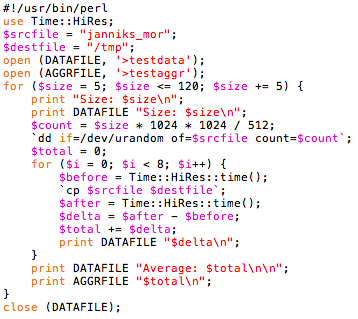
\includegraphics[width=4in]{kode.png}
	\caption{Perl-scriptet}
	\label{ploto}
\end{figure}

% 2.b
\subsection{Graf}
På figur \ref{ploto} ses 

\begin{figure}
	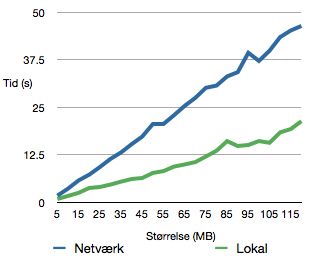
\includegraphics[width=4in]{ploto.png}
	\caption{Hastigheden for lokal og netværk.}
	\label{ploto}
\end{figure}

\begin{figure}
	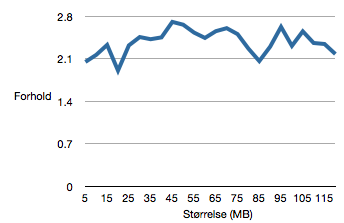
\includegraphics[width=4in]{plotforhold.png}
	\caption{Forholdet mellem de to hastigheder.}
	\label{plotforhold}
\end{figure}

% 2.c
\subsection{Teseoverlevelse}

\textit{Alt andet lige holder tesen ikke.}
Overførslen til en lokal harddisk er op til dobbelt så hurtig som til en harddisk på et lokalt netværk.
Det er muligt at det vil se anderledes ud med større filer, men ingen tendens.
Ændre rækkefølge på tests så der alterneres mellem størrelser på de overførte filer frem for at der uploades hver størrelse 10 gange efter hinanden.
Hvorfor skulle det hjælpe med større filer?

% 2.c.i
\subsubsection{i}

% 2.c.ii
\subsubsection{ii}

% 3
\section{Ræssonnering}

% 3.a
\subsection{a}

% 3.b
\subsection{b}

% 3.c
\subsection{c}

\section{Perspektivering i forhold til artikler}

Stewart er netop frustreret over en mangel på sådan rigid opstillelse af teser og be- eller akræftning af disse. Han ville derfor formentlig acceptere vores grundlæggende metode og kalde det \textit{computer science}, omend vores udførsel og faktiske planlægning af eksperimentet efterlader noget at ønske. Han synes at gå ind for Poppers forudsætninger for videnskab, som kræver formelle og falsificerbare teser og rig mulighed for ekstern afprøvning/bekræftelse. Vores eksperiment er i teorien replikerbart, men i praksis er det ikke tilnærmelsesvist grundigt nok dokumenteret: det brugte hardware er ikke specificeret, og eksempelvis netværk har en masse usikkerhed, der ikke er taget højde for.   

\end{document}
